\begin{alist}
\item Ισχύει ότι
\[f(x) = \ln\frac{1}{|x|} = \ln 1 - \ln|x| = 0 - \ln|x| = -\ln|x|.\]

\item 
\begin{rlist}
\item Η γραφική παράσταση της $f(x) = -\ln|x|$ είναι η συμμετρική της γραφικής παράστασης της $h(x) = \ln|x|$ ως προς τον άξονα $x'x$ και φαίνεται στο επόμενο σχήμα.
\begin{center}
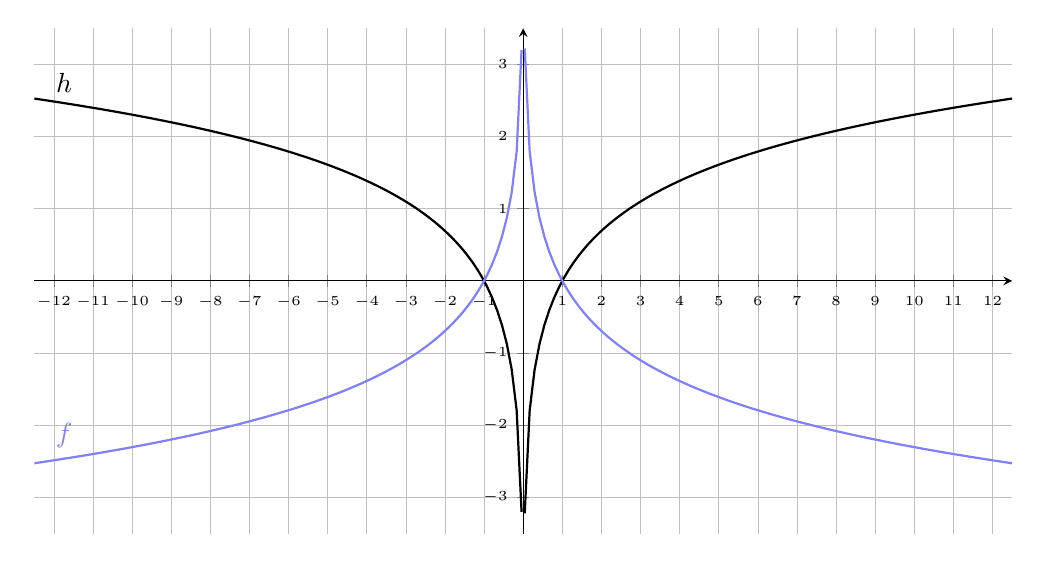
\begin{tikzpicture}
\begin{axis}[
    axis lines=middle,
    xmin=-12.5, xmax=12.5,
    ymin=-3.5, ymax=3.5,
    xtick={-12,-11,-10,-9,-8,-7,-6,-5,-4,-3,-2,-1,1,2,3,4,5,6,7,8,9,10,11,12},
    ytick={-3,-2,-1,1,2,3},
    ticklabel style={font=\tiny},
    width=14cm, height=8cm,
    samples=100,
    grid=both,
    grid style={line width=.1pt, draw=gray!20},
    major grid style={line width=.2pt,draw=gray!50}
]
\addplot[domain=0.04:12.5, thick, black] {ln(x)};
\addplot[domain=-12.5:-0.04, thick, black] {ln(-x)} node[pos=0.05, above] {$h$};
\addplot[domain=0.04:12.5, thick, blue!50!white] {-ln(x)};
\addplot[domain=-12.5:-0.04, thick, blue!50!white] {-ln(-x)} node[pos=0.05, above] {$f$};
\end{axis}
\end{tikzpicture}
\end{center}

\item Οι γραφικές παραστάσεις των $f, g$ έχουν μοναδικό κοινό σημείο, διότι, πρέπει να ισχύει:
\[f(x) = g(x) \Leftrightarrow -\ln|x| = \ln x, x > 0 \Leftrightarrow -\ln x = \ln x \Leftrightarrow 0 = 2\ln x \Leftrightarrow \ln x = 0 \Leftrightarrow x = 1.\]
Αυτό φαίνεται και στο επόμενο σχήμα:
\begin{center}
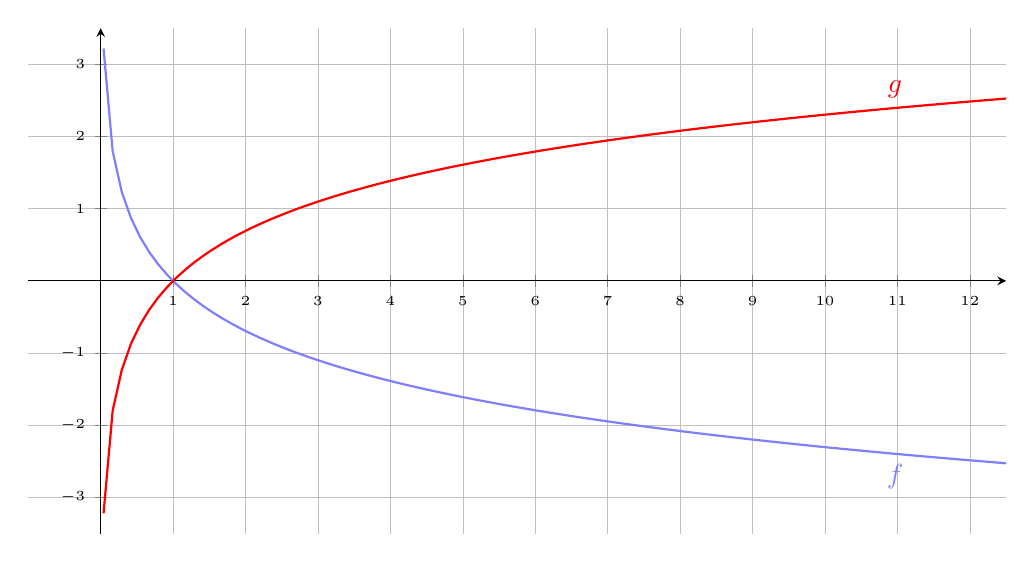
\begin{tikzpicture}
\begin{axis}[
    axis lines=middle,
    xmin=-1, xmax=12.5,
    ymin=-3.5, ymax=3.5,
    xtick={1,2,3,4,5,6,7,8,9,10,11,12},
    ytick={-3,-2,-1,1,2,3},
    ticklabel style={font=\tiny},
    width=14cm, height=8cm,
    samples=100,
    grid=both,
    grid style={line width=.1pt, draw=gray!20},
    major grid style={line width=.2pt,draw=gray!50}
]
\addplot[domain=0.04:12.5, thick, blue!50!white] {-ln(x)} node[pos=0.9, below] {$f$};
\addplot[domain=0.04:12.5, thick, red] {ln(x)} node[pos=0.9, above] {$g$};
\end{axis}
\end{tikzpicture}
\end{center}
\end{rlist}
\end{alist}
